% !TeX program = xelatex
% Standalone, source-grounded technical note. Compile twice with XeLaTeX.
\documentclass[UTF8,a4paper,11pt,fontset=windows]{ctexart}
\usepackage[margin=20mm,headheight=15pt]{geometry}
\usepackage{amsmath,amssymb,amsthm,bm}
\usepackage{graphicx,xcolor,booktabs,tabularx,array,float,caption}
\usepackage{fancyhdr,hyperref}
\setmainfont{Times New Roman}
\setsansfont{Arial}
\definecolor{navy}{HTML}{20374B}
\definecolor{blue}{HTML}{2879AD}
\definecolor{purple}{HTML}{7754A0}
\definecolor{orange}{HTML}{B67C35}
\definecolor{pale}{HTML}{EAF3F9}
\hypersetup{colorlinks=true,linkcolor=blue,citecolor=purple,urlcolor=blue,
 pdftitle={J11 柑橘幼果实例分割：数学推导、图解与证据边界},
 pdfauthor={柑橘套袋视觉研究}}
\captionsetup{font=small,labelfont=bf,labelsep=quad,skip=6pt}
\graphicspath{{figures/}}
\pagestyle{fancy}
\fancyhf{}
\fancyhead[L]{\small J11：数学推导与图解}
\fancyhead[R]{\small 实现核对版 \textperiodcentered\ 2026-10-01}
\fancyfoot[C]{\small \thepage}
\renewcommand{\headrulewidth}{0.3pt}
\ctexset{section={format=\Large\bfseries\color{navy}},
 subsection={format=\large\bfseries\color{navy}}}
\setlength{\parskip}{4pt}
\setlength{\parindent}{2em}
\setlength{\abovedisplayskip}{7pt}
\setlength{\belowdisplayskip}{7pt}
\renewcommand{\arraystretch}{1.25}
\newcolumntype{Y}{>{\raggedright\arraybackslash}X}
\newtheorem{proposition}{命题}[section]
\newtheorem{corollary}[proposition]{推论}
\renewcommand{\proofname}{证明}
\newcommand{\R}{\mathbb{R}}
\newcommand{\one}{\bm{1}}
\newcommand{\sigmoid}{\operatorname{sigmoid}}
\newcommand{\softmax}{\operatorname{softmax}}
\newcommand{\rank}{\operatorname{rank}}
\newcommand{\BCE}{\operatorname{BCE}}
\newcommand{\Pool}{\operatorname{Pool}}
\newcommand{\Up}{\operatorname{Up}}
\newcommand{\tr}{\mathsf{T}}
\newcommand{\note}[2]{\par\smallskip\noindent\fcolorbox{blue!45}{pale}{%
\begin{minipage}{\dimexpr\linewidth-2\fboxsep-2\fboxrule\relax}
\small\textbf{#1}\quad #2\end{minipage}}\par\smallskip}
\newcommand{\limitation}[1]{\par\noindent\textcolor{orange}{\textbf{适用边界：}}#1\par}
\newcommand{\fig}[4]{\begin{figure}[H]\centering
\includegraphics[width=#2\linewidth]{#1}\caption{#3}\label{#4}\end{figure}}

\begin{document}
\begin{titlepage}
\thispagestyle{empty}
\vspace*{10mm}
{\sffamily\color{blue}\large CITRUS INSTANCE SEGMENTATION\par}
\vspace{8mm}
{\Huge\bfseries\color{navy} J11 柑橘幼果实例分割\par}
\vspace{4mm}
{\LARGE\bfseries 数学推导、模块图解与证据边界\par}
\vspace{8mm}
{\large 回答三个问题：为什么这样设计？\par
哪些性质能够证明？还需要哪些实验？\par}
\vspace{8mm}
\noindent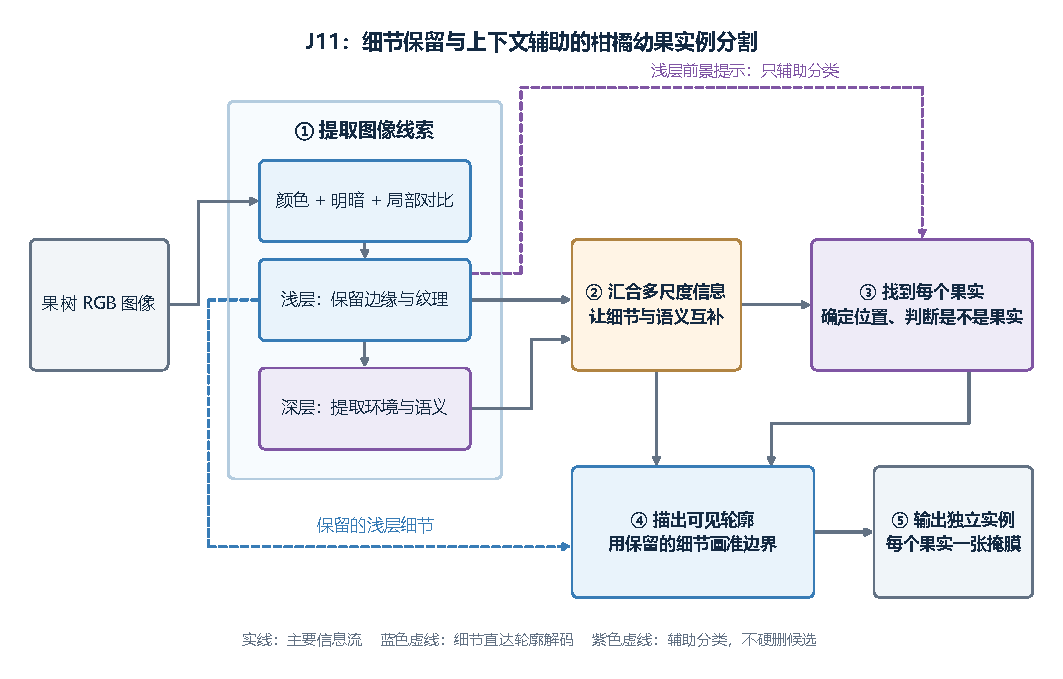
\includegraphics[width=\linewidth]{01_architecture_overview.pdf}
\vspace{5mm}
\note{阅读前提}{J11 是当前结构完整、预算较低的\textbf{综合候选}，不是已证实的精度冠军。
本文件不把代数性质等同于 mAP 提升，也不把旧验证集成绩当正式测试集结论。
图中“找到”“保留”等措辞表示设计目的，不表示目标已经达成。}
\vfill
{\large 面向 RGB 未成熟柑橘\textbf{可见实例掩膜}，不补全遮挡部分\par}
{\small 源码核对日期：2026 年 10 月 1 日\quad 排版：XeLaTeX\par}
\end{titlepage}

\section*{先给结论：强在哪里，为什么暂时不能说“最强”}
\addcontentsline{toc}{section}{结论与阅读说明}
J11 最值得研究的并不是又增加了一种注意力，而是把有限计算分给不同任务：
\textbf{低通道浅层保留空间细节；检测分支在 P3/P4/P5 建立实例；P1/P2 直接支撑轮廓解码；
深层上下文仅作有界残差修正。}这是一种可检验的任务分流结构。

\begin{table}[H]\centering\small
\caption*{本文件能够支持的判断，与不能越过的证据边界}
\begin{tabularx}{\linewidth}{p{30mm}YY}
\toprule
设计机制 & 可严格推导的性质 & 不能由此推出的结论\\
\midrule
相位重排入口 & 重排算子是可逆置换 & 重排后压缩、整个主干都无损\\
局部对比线索 & 对公共亮度偏移不变 & 灰度增加信息，或解决所有绿色混淆\\
竞争式融合 & 混合前的凸包界及显式权重梯度 & 全网络非扩张，或弱小目标必被增强\\
差分上下文 & 公共常量分量消除，读取代价与槽数有关 & 所有树叶被消除，或果实一定保留\\
浅层原型解码 & 更细原型栅格；线性 logits 秩上界 & 自动获得新候选，或高分辨率必涨点\\
有界修正 & 相对残差系数有界、初始恒等 & 训练全局收敛，或优化器具有 PID 稳定性\\
\bottomrule
\end{tabularx}
\end{table}

本地统一输入 \(640\times640\)、单类构建诊断得到 J11 参数约 \(1.075\) M、估算计算量
\(5.216\) GFLOPs；匹配内部对照 J00 为 \(2.843\) M、\(10.356\) GFLOPs。
但同一次 \textbf{CPU} 微基准的前向中位耗时是 \(123.1\) ms 对 \(118.8\) ms，
因此\textbf{低参数、低 FLOPs 已有证据，“更快”和“精度最高”没有证据}。
这是当前最重要的结论边界。

\subsection*{如何阅读}
每项核心设计按“实际公式—命题—证明—任务意义—反例”展开。
\textcolor{blue}{蓝色框}给出直观解释；\textcolor{orange}{橙色提示}给出不能过度解读的条件。
解析示意图不是训练曲线；历史诊断图与 J11 的成绩严格分开。
文末列出可直接用于实验验证的比较关系和参考文献。

\clearpage
\setcounter{tocdepth}{1}
\tableofcontents
\clearpage

\section{任务定义与证据：先解释为什么极小目标困难}
\label{sec:geometry}
设 RGB 图像为 \(X\in\R^{3\times H\times W}\)，标注为可见实例集合
\(\mathcal G=\{(b_i,M_i)\}_{i=1}^{n}\)，其中
\(M_i\in\{0,1\}^{H\times W}\) 不包含被叶枝遮挡、无法看见的区域。
模型预测 \(\{(\hat b_j,s_j,\hat M_j)\}\)，需要同时完成候选发现、分数排序和掩膜拟合。
\textbf{“绿色相近”是混淆假设，不是仅凭颜色相近就已证明的错误归因。}

\subsection{像素误差的尺度放大效应}
\begin{proposition}[同尺寸方形掩膜的平移敏感性]\label{prop:iou}
两个边长为 \(d>0\) 的方形掩膜沿横、纵方向同时相差 \(\delta\)，且
\(0\leq\delta\leq d\)，则
\begin{equation}
\operatorname{IoU}(d,\delta)
=\frac{(d-\delta)^2}{2d^2-(d-\delta)^2}.
\label{eq:iou}
\end{equation}
若要求 \(\operatorname{IoU}\geq\tau\)，其中 \(0<\tau<1\)，则充要条件为
\begin{equation}
\frac{\delta}{d}\leq 1-\sqrt{\frac{2\tau}{1+\tau}}.
\label{eq:tol}
\end{equation}
\end{proposition}
\begin{proof}
交集面积为 \((d-\delta)^2\)，并集面积为两方形面积之和减交集，得到式\eqref{eq:iou}。
记 \(r=\delta/d\)，则 \((1-r)^2/[2-(1-r)^2]\geq\tau\) 等价于
\((1-r)^2\geq2\tau/(1+\tau)\)。由于 \(1-r\geq0\)，取非负平方根即得式\eqref{eq:tol}。
\end{proof}
当 \(\tau=0.5\) 时，允许相对偏移仅约 \(18.35\%\)。
\(\delta=1\) 像素时，\(d=4,8,16\) 对应 IoU 分别为
\(9/23\approx0.391\)、\(49/79\approx0.620\)、\(225/287\approx0.784\)。

\fig{02_small_geometry.pdf}{1}{(a) 方形掩膜解析曲线，不是模型成绩；
(b) 正式 grouped\_dedup 划分在静态 letterbox640 下的 GT 短边比例。
训练集 4,120 个、验证集 1,181 个实例；没有增强、没有预测，也不代表召回。}{fig:geometry}

\note{对本任务的含义}{应减少输入缩小、边界栅格和实例合并造成的相对误差；
但仅仅把输出原型做细，不能恢复输入里已经不可区分的目标，也不能替代候选发现。}
\limitation{真实果实有深凹可见轮廓和遮挡，不是方形；上述精确公式是敏感性分析，不是实际 AP 定律。
静态几何审计也不能替代增强后标签分配和难例诊断。}
\clearpage

\section{J11 的真实计算图与符号}
\label{sec:graph}
下表直接对应 \texttt{J11\_synthesis.yaml}。批量维度省略，\(C_k\) 表示主干特征，
\(P_k\) 表示送给头部的融合特征；二者不要混用。
\begin{table}[H]\centering\small
\caption{J11 在 640 输入、单类任务下的张量契约}
\begin{tabularx}{\linewidth}{p{19mm}p{27mm}Y}
\toprule
符号 & 形状：通道\(\times\)空间 & 对应操作与任务\\
\midrule
\(C_1\) & \(16\times320^2\) & RGB/亮度/局部对比，相位重排入口；保留早期细节\\
\(C_2\) & \(32\times160^2\) & JDown + JStage\(\times2\)；掩膜细节及场景监督\\
\(C_3\) & \(64\times80^2\) & JDown + JStage\(\times2\)；检测尺度 8\\
\(C_4\) & \(96\times40^2\) & JDown + JStage\(\times3\) + JContext；上下文尺度 16\\
\(C_5\) & \(160\times20^2\) & JDown + JStage\(\times2\) + SPPF；深层语义\\
\(P_3\) & \(64\times80^2\) & \(\mathcal F_3(C_3,C_2,C_4)\)\\
\(P_4\) & \(96\times40^2\) & \(\mathcal F_4(C_4,C_3,C_5)\)\\
\(P_5\) & \(128\times20^2\) & \(\mathcal F_5(C_5,C_4)\)\\
\(\mathcal P\) & \(32\times320^2\) & \(C_2+P_3\) 的语义细节与 \(C_1\) 合成原型\\
\bottomrule
\end{tabularx}
\end{table}

\subsection{结构上的关键变化}
\begin{equation}
(C_1,C_2,C_3,C_4,C_5)=\mathcal E(X),\qquad
P_k=\mathcal F_k(\mathcal S_k),\quad k\in\{3,4,5\}.
\label{eq:graph}
\end{equation}
JStage 不是原版 C3k2/CSP 堆叠；颈部从各主干尺度\textbf{分别读取并一次式融合}，
没有重复完整的自顶向下、自底向上 PAN 路径。
头部的框、分类和实例系数仍复用 Ultralytics 的检测接口；掩膜原型采用独立细节路径。
\textbf{这是新的编码和融合设计，但不是摆脱所有 YOLO 实现依赖的完全独立框架。}

\begin{equation}
N_{\mathrm{cand}}=80^2+40^2+20^2=8400.
\label{eq:candidate}
\end{equation}
\(C_1/C_2\) 参与掩膜或场景支路，\textbf{没有}增加 stride 2/4 的检测候选。
因此本文不能把细节分支描述成“全程高分辨率检测主线”或“已有 P2 小目标检测头”。

\note{为什么选择它来讲推导}{它同时具备细节入口、低通道非 CSP 主干、不同尺度的直接融合、
有限槽位上下文和独立轮廓解码，适合分析计算如何服务本任务。
综合性是选择理由，不是精度排名的证据。}
\clearpage

\section{入口推导：灰度与局部对比，增加的是归纳偏置}
\label{sec:stem}
实际亮度通道为
\begin{equation}
Y(p)=0.2989X_R(p)+0.5870X_G(p)+0.1140X_B(p),\qquad
Q(p)=Y(p)-\frac{1}{|\mathcal N_p|}\sum_{q\in\mathcal N_p}Y(q).
\label{eq:gray}
\end{equation}
\(\mathcal N_p\) 是 \(5\times5\) 邻域与有效图像区域的交集。
实现使用 \texttt{count\_include\_pad=False}，边界处也按有效像素计均值。
入口拼接为 \(Z=[X,Y,Q]\in\R^{5\times H\times W}\)。

\begin{proposition}[局部对比的公共亮度偏移不变性]
对任意常量 \(a\)，定义 \(Y'(p)=Y(p)+a\)。如果邻域平均的权重和为 1，
则 \(Q'(p)=Q(p)\)，包括采用有效像素归一化的边界位置。
\end{proposition}
\begin{proof}
\(Q'(p)=Y(p)+a-|\mathcal N_p|^{-1}\sum_q(Y(q)+a)
=Y(p)-|\mathcal N_p|^{-1}\sum_qY(q)=Q(p)\)。
\end{proof}
此性质针对\textbf{亮度域的公共加法偏移}，不是对曝光缩放、局部阴影、饱和裁剪或任意色变都不变。
灰度转化也可能压低仅由色度体现的果叶差异，因此 RGB 始终保留。

\begin{proposition}[确定性附加通道不会凭空增加信息]
设目标随机变量为 \(T\)，\(g(X)=(Y,Q)\) 为 RGB 的确定性函数。
在相关互信息存在的条件下，
\begin{equation}
I(T;X,g(X))=I(T;X).
\label{eq:information}
\end{equation}
\end{proposition}
\begin{proof}
互信息链式法则给出 \(I(T;X,g(X))=I(T;X)+I(T;g(X)\mid X)\)。
给定 \(X\) 后 \(g(X)\) 已确定，条件互信息为零。
\end{proof}

\note{为什么仍可能有用}{不是给模型额外传感器，而是把“相对明暗变化”显式放到可读取的通道，
减少低预算网络自行学出同类滤波的负担。这个优化和泛化假设必须由
J05 与 J06 的同协议实验、颜色扰动及果叶误报统计验证。}

\subsection{可发表的准确表述}
可写“引入显式的无色度细节归纳偏置”，不能写“增加新的物理信息”或
“数学证明灰度比 RGB 更强”。这里只提出针对任务的表示方式；与 RGB 的互补性尚待实测。
\clearpage

\section{下采样推导：可逆重排与不可逆压缩要分开}
\label{sec:phase}
当 \(H,W\) 为偶数，定义空间到通道的相位重排 \(\mathcal U\)：
\begin{equation}
[\mathcal U(Z)]_{4c+2a+b,i,j}=Z_{c,2i+a,2j+b},\qquad a,b\in\{0,1\}.
\label{eq:shuffle}
\end{equation}
它将 \(C\times H\times W\) 变为 \(4C\times H/2\times W/2\)，元素总数不变。
JStem 模式 2 先把 5 通道重排为 20 通道，再学习投影到 16 通道；
JDown 同样先重排，再执行 \(1\times1\) Conv-BN-SiLU 投影。

\fig{03_phase_rearrangement.pdf}{1}{原创相位示意。a、b、c、d 代表相邻空间位置，
不是四个独立语义。可逆的是重排本身，右侧学习压缩不继承可逆保证。}{fig:phase}

\begin{proposition}[重排是等距置换]
将张量向量化后，\(\mathcal U\) 对应置换矩阵 \(U\)，满足
\begin{equation}
U^\tr U=I,\qquad U^{-1}=U^\tr,\qquad \|Uz\|_2=\|z\|_2.
\end{equation}
\end{proposition}
\begin{proof}
式\eqref{eq:shuffle}为每个输入元素建立唯一输出索引，反向索引唯一。
置换矩阵每行、每列恰有一个 1，其余为 0，所以正交；范数结论随即成立。
\end{proof}

\begin{proposition}[学习压缩的非单射条件]
令 \(W\in\R^{C_{\mathrm{out}}\times4C}\)。若存在非零 \(v\in\ker W\)，
并且 \(z,z+v\) 均属于允许输入域，则 \(Wz=W(z+v)\)。任何仅作用于 \(Wz\) 的后续变换均无法区分两者。
\end{proposition}
\begin{proof}由线性性，\(W(z+v)=Wz+Wv=Wz\)。施加相同后续函数仍相等。\end{proof}
当 \(C_{\mathrm{out}}<4C\) 时，秩-零化度定理保证在完整特征空间有非平凡核。
例如 \(W=[1\;1]\)，\(v=[1\;-1]^\tr\) 被完全抹去。
\limitation{入口的 Y/Q 是 RGB 的确定性冗余；20 到 16 通道\textbf{不能仅凭维数}就证明
真实 RGB 流形上必有信息丢失。JDown 的完整特征域则仍具有上述压缩风险。
准确主张是“压缩前保留四相位供学习选择”，不是“整个主干无损”。}
\clearpage

\section{轻量主干推导：空间混合便宜，不代表整网更快}
\label{sec:stage}
对 \(F\in\R^{C\times h\times w}\)，设 \(a=\lfloor C/4\rfloor\)，
将通道分为 \(F_A,F_B\)。JStage 内单个实际残差块为
\begin{align}
\widetilde F &= [\operatorname{Conv}_{3\times3}(F_A),F_B],\notag\\
V &= \operatorname{Conv}_{1\times1}(\widetilde F),\qquad
G=\sigmoid\!\left(W_g\operatorname{DWConv}_{5\times5}(\widetilde F)+b_g\right),\notag\\
F^+&=F+\tanh(\bm g)\odot\operatorname{Conv}^{\mathrm{no\ act}}_{1\times1}(V\odot G).
\label{eq:jblock}
\end{align}
其中 Conv 包含代码约定的 BN/激活，最后投影仅关闭激活、仍有 BN。
\(\bm g\) 为逐通道参数，初值 0.1；门 \(G\) 在 \((0,1)\)，但残差值和投影权重不受范数约束。
设计借鉴部分通道空间卷积思路\cite{fasternet}，并非 FasterNet 整网复现。

\subsection{算术复杂度}
忽略 BN、激活和逐元素操作，标准 \(3\times3\) 全通道卷积的 MAC 数为
\(9hwC^2\)。只在四分之一通道上卷积，则
\begin{equation}
\operatorname{MAC}_{\mathrm{partial}}=9hwa^2
\approx\frac{1}{16}\,9hwC^2.
\label{eq:pcost}
\end{equation}
\textbf{这仅是空间卷积分量的节省，不是整个块节省 16 倍。}
式\eqref{eq:jblock}还包含三个 \(C\to C\) 点卷积和一个深度卷积，约为
\begin{equation}
\operatorname{MAC}_{\mathrm{block}}
\approx hw\left(9a^2+3C^2+25C\right).
\label{eq:blockcost}
\end{equation}
本文 FLOPs 诊断采用乘加算 2 次浮点操作的惯例，并另补 JContext 矩阵乘部分。
未计池化、插值、张量重排、所有非线性与数据搬运，所以为\textbf{估算值}，不是硬件性能证明。

\begin{table}[H]\centering\small
\caption{本地 CPU 构建诊断；不是训练结果，也不是 GPU 推理测试}
\begin{tabular}{lrrr}\toprule
模型 & 参数 / M & 估算 GFLOPs & CPU 前向中位时间 / ms\\\midrule
J00 匹配内部对照 & 2.843 & 10.356 & 118.8\\
J11 综合候选 & 1.075 & 5.216 & 123.1\\
J17 进一步压缩 & 0.709 & 3.875 & 128.1\\\bottomrule
\end{tabular}
\end{table}
\note{实际含义}{J11 参数约减少 62.2\%，估算 FLOPs 约减少 49.6\%，但此 CPU 诊断并未更快。
碎片化小算子、内存读写和调度足以抵消算术量优势；最终必须在同 GPU、同 batch、同部署路径测量。
对精度而言，轻量主干可能失去容量，需用更低预算换来的细节路径收益证明其值得。}
\clearpage

\section{颈部推导：一次式竞争融合的优点与风险}
\label{sec:fusion}
对一个目标尺度，来源特征先经点卷积投影，再按目标大小做平均池化或最近邻上采样：
\begin{equation}
V_i=\mathcal R_i(\phi_i(C_i)),\quad
\bm a(p)=W_s[V_1(p),\ldots,V_K(p)]+b_s,
\quad\alpha_i(p)=\frac{e^{a_i(p)}}{\sum_j e^{a_j(p)}}.
\label{eq:fusionweights}
\end{equation}
\(\phi_i\) \textbf{在重采样之前}执行，这与“先上采样，再投影”的成本、数值行为不同。
实际输出为
\begin{equation}
F(p)=\sum_{i=1}^{K}\alpha_i(p)V_i(p),\qquad
P=\psi_{\mathrm{DW3+PW1}}(F).
\label{eq:fusion}
\end{equation}
空间自适应尺度权重已有 ASFF 先例\cite{asff}；本文可研究的重点是\textbf{低预算直接拓扑和任务分流}，
不能把 softmax 加权本身宣称为首次提出。

\fig{04_competitive_fusion.pdf}{1}{(a) 每个目标尺度从主干直接读取；
(b) 人工数值示例：细节源响应为 1，其余两个源为 0.1，细节权重为 \(1/3\) 时混合响应为 0.4。
曲线不是训练权重或真实果实激活。}{fig:fusion}

\begin{proposition}[精炼前的凸包界与竞争梯度]
固定各源值 \(V_i(p)\)，则 \(F(p)\) 属于其凸包，任意范数满足
\begin{equation}
\|F(p)\|\leq\sum_i\alpha_i(p)\|V_i(p)\|\leq\max_i\|V_i(p)\|.
\label{eq:convexbound}
\end{equation}
对任一权重 logit \(a_j\) 有
\begin{equation}
\frac{\partial F}{\partial a_j}=\alpha_j(V_j-F).
\label{eq:fusiongrad}
\end{equation}
\end{proposition}
\begin{proof}
softmax 产生非负且和为 1 的权重，因此为凸组合，范数不等式由三角不等式得到。
由 \(\partial\alpha_i/\partial a_j=\alpha_i(\mathbf1_{i=j}-\alpha_j)\)，代入式\eqref{eq:fusion}即得梯度。
\end{proof}
若上游损失梯度为 \(h=\partial\mathcal L/\partial F\)，则
\(\partial\mathcal L/\partial a_j=\alpha_j\langle h,V_j-F\rangle\)，说明权重可学习是否需要某来源。
\limitation{这个方向由损失决定，不等于网络知道“哪个是果实”。零初始化的权重是均匀混合，
可能稀释仅一个尺度可见的微弱目标。}\clearpage

\section{融合为何不等于抗混叠或全网稳定}
\label{sec:fusionlimits}
\subsection{输入导数不是简单的凸平均}
当来源和权重都依赖输入 \(x\) 时，完整导数为
\begin{equation}
\frac{\partial F}{\partial x}
=\sum_i\alpha_i\frac{\partial V_i}{\partial x}
+\sum_iV_i\frac{\partial\alpha_i}{\partial x}.
\label{eq:fullfusionjac}
\end{equation}
第二项不能省略；\(P=\psi(F)\) 还引入学习投影的导数。
因此凸包界\eqref{eq:convexbound}不是输入扰动非扩张证明，不是全网 Lipschitz 常数小于 1 的证明。

\subsection{平均池化对稀疏信号的稀释}
设一个池化窗有 \(m\) 个位置，其中只有 \(r\) 个位置含幅值 \(A\) 的额外目标响应，
其余为同一背景 \(B\)。则平均池化为
\begin{equation}
\overline V=B+\frac{r}{m}A.
\label{eq:pooldilution}
\end{equation}
\(r\ll m\) 时，该来源的目标残差幅值按占比减小；这是明确反例。
最大池化有不同的信息偏置，最近邻上采样不创造新的真实边界；没有某个简单算子自动同时解决所有问题。
频率感知融合研究\cite{freqfusion}提供了可研究方向，但 J11\textbf{没有}实现其频率估计、
自适应滤波或位移校正，不能引用其整套性质给当前 JFusion 背书。

\subsection{一次式直接融合的合理研究假设}
\begin{equation}
C_i\longrightarrow P_k\longrightarrow\text{实例头},
\quad\text{而不是反复经过多轮融合才读出浅层信息。}
\end{equation}
更短的信息路径可能减少重复变换造成的细节稀释；较少高分辨率中间节点可能降低计算预算。
\textbf{“路径更短”是结构事实，“信号更好”仍是实验假设}：来源不一致、空间错位、投影瓶颈、均匀初值都可能使其失败。

\note{最有价值的验证}{不要只看总 mAP。比较 J05 的均匀融合与 J08 的竞争融合，
统计超小目标召回、果叶误报、权重熵和失败样例；再比较同预算普通 PAN 与直接拓扑。
若只替换模块却不控制主干、掩膜分辨率和训练协议，就不能归因到融合方式。}
\clearpage

\section{上下文推导：有限槽位差分读取的可证明部分}
\label{sec:context}
在 \(C_4\) 上，\(N=40^2=1600\)，通道投影维度 \(d=16\)，
上下文池化到 \(4\times4\)，故记忆槽数 \(m=16\)。令
\(Q_1,Q_2\in\R^{N\times d}\)，\(K_1,K_2,V\in\R^{m\times d}\)。实际读取为
\begin{align}
A_1&=\softmax\!\left(Q_1K_1^\tr/\sqrt d\right),\qquad
A_2=\softmax\!\left(Q_2K_2^\tr/\sqrt d\right),\notag\\
D&=A_1-A_2,\qquad R=DV,\qquad
F^+=F+0.25\tanh(g)W_oR.
\label{eq:diff}
\end{align}
softmax 沿记忆槽方向执行，\(g\) 初值为 0。借鉴差分注意力及压缩视觉对比思想\cite{diff,linear}，
但当前没有原论文的完整双阶段交互、位置编码、可学习差分系数或全部归一化机制。

\begin{proposition}[公共常量分量消除与有限读出界]\label{prop:diff}
在精确实数运算下，\(D\one_m=0\)。若
\(V=\one_m v_0^\tr+E\)，则
\begin{equation}
DV=DE,\qquad \|D\|_{\infty}\leq2,\qquad
\|DV\|_{\max}\leq2\|V\|_{\max},
\label{eq:null}
\end{equation}
其中 \(\|\cdot\|_\infty\) 为最大绝对行和，\(\|\cdot\|_{\max}\) 为元素绝对值的最大值。
\end{proposition}
\begin{proof}
每个概率矩阵的行和都是 1，所以 \((A_1-A_2)\one_m=0\)。
常量部分右乘后为零，得到 \(DV=DE\)。每行有
\(\sum_j|A_{1,ij}-A_{2,ij}|\leq\sum_j(A_{1,ij}+A_{2,ij})=2\)，
再逐元素应用三角不等式得到幅值界。
\end{proof}

\fig{05_differential_context.pdf}{1}{人工概率例子展示公共常量消除。
槽位 1 与 4 的局部突起产生相反符号，不代表“正值是果实、负值是叶片”。
图中槽位数为 4，便于阅读；代码使用 16。}{fig:diff}

\note{为什么值得尝试}{绿色果叶共享部分低区分度响应时，差分读取具备去公共分量的代数能力。
但这个公共分量是否对应背景，需要特征可视化和错误统计证明；真实叶片是空间变化信号。}
\clearpage

\section{差分机制的反例、复杂度和初始化}
\label{sec:contextlimits}
\subsection{不能用零行和证明“自动去叶片”}
如果果实的有效信号也在所有槽位中相同，命题\ref{prop:diff}同样会将其消去。
若 \(A_1=A_2\)，则所有 \(V\) 都得到 \(DV=0\)。因此差分读取有\textbf{语义不确定性}，
仅保证消除数学上的公共常量，不保证目标/背景分解正确。
此外，4\(\times\)4 的 C4 池化槽在 640 输入下覆盖约 160\(\times\)160 像素，
极小果实可能在池化时被式\eqref{eq:pooldilution}稀释。该支路适合辅助上下文，不应承担唯一的小目标保留任务。

\subsection{读取矩阵的计算代价}
两个 \(QK^\tr\) 需要 \(2Nmd\) 次 MAC，差分后的 \(DV\) 需要 \(Nmd\) 次 MAC，合计
\begin{equation}
\operatorname{MAC}_{\mathrm{read}}=3Nmd,
\qquad \operatorname{FLOPs}_{\mathrm{read}}\approx6Nmd.
\label{eq:attncost}
\end{equation}
代入 \(N=1600,m=d=16\) 为 \(2{,}457{,}600\) FLOPs，即约 \(0.00246\) GFLOPs。
注意力矩阵存储量为 \(O(Nm)\)，当 \(m\) 固定时对 \(N\) 线性。
\limitation{这只计算读取矩阵；Q/K/V/out 的卷积、池化和 softmax 成本仍存在。
相比\textbf{同维数同读取形式}的全 N 槽方案，矩阵项约缩为 \(m/N\)，不能据此说整网快 100 倍。}

\subsection{零初始化不是训练全过程冻结}
把 \(R_\theta(F)=W_oDV\) 记为上下文分支，则
\begin{equation}
F^+=F+0.25\tanh(g)R_\theta(F),\quad
\left.\frac{\partial F^+}{\partial\theta}\right|_{g=0}=0,\quad
\left.\frac{\partial F^+}{\partial g}\right|_{g=0}=0.25R_\theta(F).
\label{eq:zerogate}
\end{equation}
初始前向为恒等；首步分支内部梯度为零，但门参数一般仍有梯度。
本地已有构造反向检查观察到 gain 梯度 L1 约 0.137，而 q/k 梯度为 0，符合公式。
这不是训练成功保证；若门始终不打开，该分支也可能长期无贡献。

\begin{equation}
\|F^+-F\|\leq0.25\|R_\theta(F)\|.
\end{equation}
系数有界不等于 \(R_\theta\) 有界；学习权重未施加谱范数约束，因此没有全网络稳定性定理。
\clearpage

\section{掩膜推导：把空间细节与实例发现分开}
\label{sec:mask}
实际 J11 原型构造为
\begin{align}
B_2&=\phi_2(C_2)+\Up_{2}\bigl(\phi_3(P_3)\bigr),\notag\\
B_1&=[\Up_{2}(B_2),\phi_1(C_1)],\qquad
\mathcal P=\psi_{\mathrm{DW3+PW1}}(B_1).
\label{eq:proto}
\end{align}
\(\phi_2,\phi_3\) 投影到 32 通道，\(\phi_1\) 投影到 16 通道，
拼接得到 48 通道，最终得到 32 张 \(320\times320\) 原型。
系数 \(c_j\in\R^{32}\) 来自 P3/P4/P5；在原型网格上预测
\begin{equation}
L_j(p)=\sum_{k=1}^{32}c_{jk}\mathcal P_k(p),\qquad
\hat M_j=\operatorname{Crop}_{\hat b_j}\bigl(\sigmoid(L_j)\bigr).
\label{eq:mask}
\end{equation}
原型与系数分解已有 YOLACT 先例\cite{yolact}；本文重点是\textbf{细节直接进入原型的拓扑分配}，
不是声称首创线性原型解码。

\fig{06_mask_decoder.pdf}{1}{掩膜解码真实分流：C1/C2 支撑高分辨率原型，
P3/P4/P5 建立实例系数。P1/P2 不是额外检测头；一个目标没有候选时，原型不会自动输出对应实例。}{fig:mask}

\begin{proposition}[线性原型的表达秩上界]
忽略裁剪和 sigmoid，将原型向量化为 \(P\in\R^{32\times S}\)，
实例系数矩阵为 \(C\in\R^{n\times32}\)，则所有实例 logits 为 \(L=CP\)，且
\begin{equation}
\rank(L)\leq\min\{\rank(C),\rank(P)\}\leq32.
\label{eq:rank}
\end{equation}
\end{proposition}
\begin{proof}矩阵乘积的像空间包含于左因子像空间，行空间包含于右因子行空间，所以得到秩上界。\end{proof}
\limitation{该界作用于线性 logits；各实例不同裁剪和非线性阈值后的二值掩膜不继承同一秩界。
更多原型可能增加表达能力，也增加计算和拟合风险；不能说 32 张一定足够或一定不足。}
\clearpage

\section{召回上限：细原型不能单独解决候选漏检}
\label{sec:recall}
\subsection{先定义才谈“召回上限”}
设低阈值候选集合为 \(\mathcal C(X)\)。按一对一匹配，将标注拆成
\(\mathcal G_{\mathrm{avail}}\) 与 \(\mathcal G_{\mathrm{miss}}\)：前者存在可服务该实例的候选，后者不存在。
在“掩膜必须由候选生成、解码不生成额外实例”的条件下，最终正确实例数满足
\begin{equation}
N_{\mathrm{TP}}\leq|\mathcal G_{\mathrm{avail}}|,\qquad
R\leq R_{\mathrm{avail}}:=\frac{|\mathcal G_{\mathrm{avail}}|}{|\mathcal G|}.
\label{eq:upperrecall}
\end{equation}
这是由输出机制得到的\textbf{条件性计数上界}，不是用某个任意 box IoU 指标直接替代 mask 上界。
候选匹配标准必须与实例可服务的定义一致；不能把框 IoU 0.5 简单当成所有 mask IoU 0.5 的充要条件。

\subsection{小目标的损失链条要逐段定位}
\begin{equation}
\text{输入可区分性}\rightarrow\text{特征响应}\rightarrow\text{实际正样本分配}
\rightarrow\text{候选和排序}\rightarrow\text{掩膜拟合}\rightarrow\text{跨视图合并}.
\end{equation}
当前 TAL 对小目标\textbf{资格区域}做了至少 16 像素的短边扩展，回归目标仍为原框。
静态无增强 train/val 几何审计中，扩展后零资格中心实例数均为 0；
因此“P3 网格没有中心点就是现在所有漏检的原因”\textbf{不成立}。
但资格中心存在，仍不保证 top-k、对齐分数及目标竞争后实际分配到正样本。

\fig{07_paired_evidence.pdf}{1}{历史冻结权重配对诊断。
Tiny 指 640 公共栅格上可见 GT mask 面积\(<256\)；分数阈值 0.25、mask IoU 0.5、一对一匹配，分母 161。
每模型只有一个 checkpoint，未给跨 seed 误差棒。
旧验证集不是正式 grouped\_dedup 验证集；细切片包含合并规则变化，不能孤立归因于像素尺度，更不是 J11 的成绩。}{fig:evidence}

\note{已有证据的正确用途}{切片与合并可明显改变同权重的小目标召回，但增加端到端耗时。
这支持“应优先研究可见信息与候选链”的方向，不支持“增加一个模块即可复现所有提升”。
SAHI 提供了切片推理先例\cite{sahi}，切片本身不构成全新理论创新。}
\clearpage

\section{识别先验推导：软门控不是硬筛选，也不是完全解耦}
\label{sec:scene}
J11 的 C2 场景支路产生两个 logits：前景并集 \(S_f\) 与可见实例边界并集 \(S_b\)。
只将前景概率 \(\pi=\sigmoid(S_f)\) 对各检测尺度池化，并用于分类特征：
\begin{equation}
\widetilde P_k=P_k\odot\left[1+0.25\tanh(g_s)\Pool_k(\pi)\right].
\label{eq:scenegate}
\end{equation}
框与系数 tower 直接读取原来的 \(P_k\)，分类 tower 读取 \(\widetilde P_k\)；\(g_s\) 初值 0。

\begin{proposition}[前景门的相对调制范围]
在每个特征位置，\(\Pool_k(\pi)\in[0,1]\)，因此调制系数
\begin{equation}
0.75\leq1+0.25\tanh(g_s)\Pool_k(\pi)\leq1.25.
\label{eq:scenebound}
\end{equation}
且 \(g_s=0\) 时 \(\widetilde P_k=P_k\)。
\end{proposition}
\begin{proof}平均池化保持 \([0,1]\) 范围，\(\tanh(g_s)\in[-1,1]\)，乘积再平移得到区间。\end{proof}
该门不会把某位置乘为零，避免因前景支路一次失误而\textbf{直接硬删除}候选。
但分类分数仍可能下调到阈值以下，实际召回\textbf{依然可能下降}。
系数允许正负调制，不能把它写成“只增强不抑制”。

\subsection{场景监督的精确定义}
对可见掩膜 \(M_i\)，定义 \(U=\max_iM_i\)，边界并集
\(B=\max_i\mathcal B(M_i)\)，其中 \(\mathcal B\) 为 3\(\times\)3 膨胀减腐蚀。
目标先自适应最大池化到 C2 网格，实际 J11 辅助项为
\begin{equation}
\mathcal L_{\mathrm{scene}}=\BCE\left([S_f,S_b],\operatorname{MaxPool}([U,B])\right),\quad
\lambda_s=0.1.
\label{eq:sceneloss}
\end{equation}
最大池化希望保留微小正区域，但目标构造用的是训练时已有掩膜栅格；此前已消失的实例不能由最大池化找回。

\note{控制思想的准确借鉴}{把深层识别的辅助作用限制为小幅、可关闭的残差，而不是强制覆盖所有浅层细节。
这与“受限修正”的工程思维相容，但该网络没有物理被控对象、时域闭环或 PID 控制器。
PIDNet 是可引用的启发先例\cite{pidnet}，不是本网络自动获得控制理论稳定性的依据。}
\limitation{共享主干、损失梯度和 TAL 的分类-定位对齐仍把各任务耦合在一起，不能宣称完全解耦。}
\clearpage

\section{损失推导：已经实现的项与尚未使用的项}
\label{sec:loss}
\subsection{基础掩膜损失不是简单“偏向大目标的全图 BCE”}
原基础损失对匹配正样本 \(a\) 的 GT 框内像素计算 BCE，再以框面积归一化。
其结构可写作
\begin{equation}
\mathcal L_{\mathrm{base\ mask}}
\propto\sum_{a\in\mathcal A_+}
\frac{1}{|\Omega_{g(a)}|}\sum_{p\in\Omega_{g(a)}}
\BCE\bigl(L_a(p),M_{g(a)}(p)\bigr),
\label{eq:baseloss}
\end{equation}
最终还按正样本数量和官方增益归一化。
因此不能以“原损失完全没有小目标面积归一化”为设计新损失的理由。

\subsection{可选 tiny Dice 与可见边界项：J14--J16，不是 J11}
下式针对单张图像，代码最后对具有匹配实例的图像取均值。
令 \(\mathcal A_i\) 是 GT \(i\) 的匹配系数集合，先平均系数后合成概率
\(p_i=\operatorname{Crop}_{b_i}\sigmoid(\overline c_i^\tr\mathcal P)\)。
实际可选项为
\begin{align}
D_i&=1-\frac{2\sum_p p_i(p)M_i(p)+1}{\sum_pp_i(p)+\sum_pM_i(p)+1},\notag\\
w_i&=\operatorname{clip}\!\left(\sqrt{256/\max(A_i,1)},1,2\right),\notag\\
\mathcal L_{\mathrm{tiny}}&=\frac{\sum_i w_iD_i}{\sum_iw_i},\qquad
\mathcal L_{\mathrm{boundary}}=\frac1{n_+}\sum_i
\frac{\sum_{p\in\mathcal B_i\cap\Omega_i}\BCE(L_i(p),M_i(p))}
{\max(|\mathcal B_i\cap\Omega_i|,1)}.
\label{eq:auxmask}
\end{align}
\(A_i\) 为掩膜有效面积换算到输入像素后的值，\(n_+\) 是被匹配的实例数；没有匹配的 GT 不进入这些项。
\textbf{J11 的 tiny/boundary 增益都是 0；J14 为 0.25/0，J15 为 0/0.1，J16 为 0.25/0.1。}
所有版本保留标准 box、cls、DFL 和逐候选 mask 项。

\subsection{平均系数的必要反例}
针对标签 1，若两个候选 logits 分别为 \(+8,-8\)，则
\begin{equation}
\BCE\left(\frac{8-8}{2},1\right)=\log2\approx0.693,
\quad\frac{\BCE(8,1)+\BCE(-8,1)}2\approx4.000.
\label{eq:meanbce}
\end{equation}
BCE 对 logit 为凸函数，平均 logits 的辅助项可能掩盖一个非常差的候选。
基础逐候选损失仍保留，但不能证明平均系数 Dice 更强，更不能把 BCE 的 Jensen 不等式套到 Dice 上。
\limitation{GT 边界不能强制圆形或凸包填充，否则会与条带遮挡导致的深凹可见掩膜冲突。
3\(\times\)3 形态学带在 stride 2 原型上约涉及 6 个输入像素，不是精确 3 输入像素边界。}
\clearpage

\section{控制式梯度预算：有条件的一步下降推导}
\label{sec:control}
\textbf{本节是未来可选方案，不是 J11 已实现的算法。}
辅助损失大小小，并不保证辅助梯度不伤害主任务。
GradNorm、PCGrad 已研究任务梯度尺度和冲突\cite{gradnorm,pcgrad}；这里只建立可审计的局部下降条件，
不宣称首次发明梯度控制。

令主损失梯度为 \(g_m=\nabla\mathcal L_m(\theta)\)，辅助梯度为
\(g_a=\nabla\mathcal L_a(\theta)\)，普通梯度下降一步为
\begin{equation}
\theta^+=\theta-\eta(g_m+\lambda g_a).
\label{eq:gd}
\end{equation}
一阶主损失变化近似为
\begin{equation}
\Delta\mathcal L_m\approx-\eta\|g_m\|_2^2
-\eta\lambda\langle g_m,g_a\rangle.
\label{eq:dotgradient}
\end{equation}
若内积为负，辅助梯度可能抵消主任务下降，不能仅凭同号损失增益断言有益。

\begin{proposition}[有界辅助梯度下的主损失一步下降]\label{prop:budget}
假设 \(\mathcal L_m\) 在相关线段上具有 \(\beta\)-Lipschitz 连续梯度，
\(g_m\ne0\)，\(\lambda\geq0\)，且
\(\lambda\|g_a\|_2\leq\gamma\|g_m\|_2\)，其中 \(0\leq\gamma<1\)。
若步长满足
\begin{equation}
0<\eta<\frac{2(1-\gamma)}{\beta(1+\gamma)^2},
\label{eq:stepsize}
\end{equation}
则普通梯度下降式\eqref{eq:gd}满足 \(\mathcal L_m(\theta^+)<\mathcal L_m(\theta)\)。
\end{proposition}
\begin{proof}
下降引理给出
\(\Delta\mathcal L_m\leq-\eta\langle g_m,g_m+\lambda g_a\rangle+
(\beta\eta^2/2)\|g_m+\lambda g_a\|_2^2\)。
由 Cauchy--Schwarz 和三角不等式，上界进一步为
\begin{equation}
\Delta\mathcal L_m\leq
\left[-\eta(1-\gamma)+\frac{\beta\eta^2}{2}(1+\gamma)^2\right]\|g_m\|_2^2.
\label{eq:descentbound}
\end{equation}
式\eqref{eq:stepsize}使括号严格为负，结论成立。
\end{proof}
\fig{09_gradient_budget.pdf}{0.90}{解析允许步长区域；不是训练结果。
辅助梯度预算增大时，最坏情形的安全步长缩小。}{fig:control}
\limitation{这个结论不直接适用于带动量 SGD、AdamW、自适应预条件、随机小批量、跳变分配或全局收敛。
\(\beta\) 通常未知，不能把图中的上界直接当现成超参数。真正实现前应测量冲突和开销；主梯度为零时也需单独处理。}
\clearpage

\section{PR 末端推导：横轴不是置信度，零补齐不是新的观测}
\label{sec:pr}
将候选按置信度降序排列，前 \(k\) 个候选的真阳性和假阳性为 \(T_k,F_k\)，
有 \(N_{\mathrm{GT}}\) 个真实实例，则
\begin{equation}
P_k=\frac{T_k}{T_k+F_k},\qquad R_k=\frac{T_k}{N_{\mathrm{GT}}}.
\label{eq:pr}
\end{equation}
PR 图横轴是 \textbf{Recall}，不是 confidence。
横轴在 0.85 左右跌落不能解释为“置信度 0.85 导致精度突然为零”。
应另看 Precision--Confidence、Recall--Confidence 曲线和原始 TP/FP。

\subsection{当前实现的端点约定}
已核对本地 \texttt{metrics.py} 与当日 Ultralytics 官方 main 源码\cite{ultrametrics}，
AP 辅助数组结构为
\begin{equation}
\texttt{mrec}=[0,R_1,\ldots,R_{\max},R_{\max},1],\qquad
\texttt{mpre}=[1,P_1,\ldots,P_K,0,0].
\label{eq:endpoints}
\end{equation}
重复 \(R_{\max}\) 对应人为加入的零端点；其后取单调包络并插值积分。
所以最高观测召回之后贴零的部分可能主要由\textbf{端点补齐}呈现，
不能把它逐点解释为“这些召回水平真的评估到了零精度”。

\fig{08_pr_endpoint.pdf}{1}{人工观测点仅到 Recall=0.8。
灰色虚线解释零端点补齐，不表示真实新增观测，也不是 J11 或其他模型的实际 PR。}{fig:pr}

\subsection{真正需要优化的是哪些量}
\(R_{\max}<1\) 仍意味着在当前候选生成、IoU 匹配与推理协议下有 GT 未找回。
原因可能是输入细节、目标混淆、候选过滤、掩膜不达 IoU 或合并错误。
小目标是\textbf{重要候选原因}，但需要尺度分层 TP/FN 证明，而不能仅从末端形状定性。

\note{严禁把曲线画好看当解决问题}{不删除零段、不改变端点来刷 AP、不把内部栅格 AP 冒充 COCOeval。
正式比较用相同的官方评估器和设置；重点报告低阈值召回上限、极小目标 recall、固定 precision 下的 recall、
mask AP50/50--95 及 split/merge 错误。美化端点不能修复漏检。}
\clearpage

\section{哪些优势已有证据，哪些必须通过消融证实}
\label{sec:conclusion}
\subsection{当前可保留的三条研究主线}
\textbf{一，细节与实例语义的任务分流。} 小目标误差敏感性有精确推导；
细节进入掩膜原型的结构事实可核对；历史配对诊断支持输入/推理尺度的重要性。
但候选仍在 P3/P4/P5，不能把 mask 更细当成召回问题已经解决。

\textbf{二，低预算的一次式竞争融合。} 有明确的凸组合性质和可解释的权重梯度；
相比模块反复堆叠，更容易隔离来源和测量路径代价。
然而 ASFF 已有同类权重思想，真正贡献应来自任务约束下的拓扑、预算分配和可靠消融。

\textbf{三，有限记忆的差分上下文与受限识别修正。}
零行和带来公共分量消除，固定槽数降低读取矩阵复杂度；软门不直接硬删除候选。
但公共分量不等于叶片，先验不等于正确识别；应保留反例和无差分对照。

\begin{table}[H]\centering\small
\caption{直接对应现有 J 系列的最小可归因验证关系}
\begin{tabularx}{\linewidth}{p{27mm}YY}\toprule
比较 & 隔离的主要因素 & 应读取的指标，而非只看总 AP\\\midrule
J00 与 J11 & 同协议系统收益 & mask AP50/50--95、R、参数、GPU 端到端耗时\\
J05 与 J06 & 亮度/局部对比入口 & 果叶误报、颜色扰动、尺度 R\\
J05 与 J08 & 竞争权重与均匀融合 & 小目标 R、权重熵、融合失败样例\\
J11 与 J12 & 场景支路及监督 & 分类误报、固定 precision 的 R\\
J11 与 J13 & 差分与普通读取 & 背景误报、tiny R、上下文图\\
J11/J14/J15/J16 & tiny/边界损失项 & mask AP、Boundary F1、GT 无正样本率\\
\bottomrule\end{tabularx}
\end{table}

正式结论需在 grouped\_dedup 的相同 train/val 划分、初始化、优化器、学习率、图像尺寸、AMP、
增强、掩膜栅格与评估协议下比较；主基线和最终方法各三 seed，保留独立 test 作最终确认。
J 系列的 scratch、AMP=false、mask\_ratio=2、copy\_paste=0.3 及混合输入是\textbf{协议的一部分}，
不能与旧 78/83 分基线直接做结构因果比较。

\note{最终回答}{J11 有值得验证的机制，也已有低参数、低估算 FLOPs 的实现证据。
本文数学能够证明的是算子性质、误差敏感性、表达限制和条件性优化边界；
\textbf{不能证明 AP、召回必提高，更不能证明它已经是最强模型。}
能发论文的“强”必须由同协议多 seed、难例机制和硬件实测共同兑现，而不是由图复杂或公式多来决定。}
\clearpage

\section*{参考文献：思想来源与实现差异}
\addcontentsline{toc}{section}{参考文献}
\small
以下主要链接指向论文或官方来源。数学证明由本文独立展开；引用不代表复制原论文的完整网络，
也不代表原论文在其他数据集上的增益可直接迁移到柑橘。
\begin{thebibliography}{99}
\bibitem{fasternet} Chen J, Kao S-h, He H, et al.
\textit{Run, Don't Walk: Chasing Higher FLOPS for Faster Neural Networks}. CVPR, 2023.
\href{https://arxiv.org/abs/2303.03667}{论文与元数据}；
\href{https://github.com/JierunChen/FasterNet}{作者代码}。部分通道空间处理的先例，不是当前 JStage 的完整实现。
\bibitem{asff} Liu S, Huang D, Wang Y.
\textit{Learning Spatial Fusion for Single-Shot Object Detection}. arXiv:1911.09516, 2019.
\href{https://arxiv.org/abs/1911.09516}{原论文}。空间自适应尺度融合的先例。
\bibitem{linear} Pu Y, Ying J, Li Q, et al.
\textit{Linear Differential Vision Transformer: Learning Visual Contrasts via Pairwise Differentials}.
NeurIPS, 2025. \href{https://arxiv.org/abs/2511.00833}{原论文}；
\href{https://github.com/LeapLabTHU/LinearDiff}{作者代码}。原方法具有完整视觉对比结构，JContext 为简化任务改写。
\bibitem{diff} Ye T, Dong L, Xia Y, et al.
\textit{Differential Transformer}. ICLR, 2025.
\href{https://arxiv.org/abs/2410.05258}{原论文}。差分注意力思想先例；当前固定差分系数为 1。
\bibitem{yolact} Bolya D, Zhou C, Xiao F, Lee Y J.
\textit{YOLACT: Real-Time Instance Segmentation}. ICCV, 2019.
\href{https://arxiv.org/abs/1904.02689}{原论文}。原型和实例系数的分解先例。
\bibitem{freqfusion} Chen L, et al.
\textit{Frequency-aware Feature Fusion for Dense Image Prediction}. arXiv:2408.12879, 2024.
\href{https://arxiv.org/abs/2408.12879}{原论文}；
\href{https://github.com/ying-fu/FreqFusion}{作者代码}。当前 JFusion 未实现其完整频率感知与校正机制。
\bibitem{sahi} Akyon F C, Altinuc S O, Temizel A.
\textit{Slicing Aided Hyper Inference and Fine-tuning for Small Object Detection}.
ICIP, 2022. \href{https://arxiv.org/abs/2202.06934}{原论文}；
\href{https://github.com/obss/sahi}{作者代码}。
\bibitem{pidnet} Xu J, Xiong Z, Bhattacharyya S P.
\textit{PIDNet: A Real-Time Semantic Segmentation Network Inspired by PID Controllers}.
CVPR, 2023. \href{https://arxiv.org/abs/2206.02066}{原论文}。
当前网络未实现 PID 控制器；受限残差只作为设计类比。
\bibitem{gradnorm} Chen Z, Badrinarayanan V, Lee C-Y, Rabinovich A.
\textit{GradNorm: Gradient Normalization for Adaptive Loss Balancing in Deep Multitask Networks}.
ICML, PMLR 80:794--803, 2018. \href{https://proceedings.mlr.press/v80/chen18a.html}{正式论文}。
\bibitem{pcgrad} Yu T, Kumar S, Gupta A, et al.
\textit{Gradient Surgery for Multi-Task Learning}. NeurIPS, 2020.
\href{https://proceedings.neurips.cc/paper_files/paper/2020/hash/3fe78a8acf5fda99de95303940a2420c-Abstract.html}{正式论文}。
梯度冲突处理先例；本文的预算推导不是已经实施的 PCGrad。
\bibitem{ultrametrics} Ultralytics.
\textit{ultralytics/utils/metrics.py}, official main source.
\href{https://github.com/ultralytics/ultralytics/blob/main/ultralytics/utils/metrics.py}{官方源文件}。
核对日期 2026-10-01；正式实验应冻结具体版本。
\end{thebibliography}
\normalsize
\clearpage

\section*{附录：复核入口、数学检查与来源账本}
\addcontentsline{toc}{section}{复核与来源账本}
\subsection*{实现与证据文件}
下列路径相对主工作副本 \texttt{1\_SEVER/code/ultralytics-main-new/}：
\begin{itemize}
\item \texttt{0\_orange\_yaml/J\_series/J11\_synthesis.yaml}：完整结构与头部损失参数。
\item \texttt{ultralytics/nn/modules/citrus\_j.py}：入口、主干、融合、上下文、实例头。
\item \texttt{ultralytics/utils/citrus\_j\_loss.py}：场景与可选 tiny/边界损失。
\item \texttt{docs/J\_STRICT\_REVIEW\_20261001/REPORT.md}：历史结果、数据与研究假设重审。
\end{itemize}
数据来源为工作区 \texttt{\_work/} 下的三个诊断产物：
\begin{itemize}
\item \texttt{20261001\_j\_strict\_review\_v3/audit.json}：正式划分几何、符号检查与反例。
\item \texttt{20261001\_j/evidence/bounded\_evidence.json}：历史冻结权重配对诊断。
\item \texttt{20261001\_j/profile/model\_costs.csv}：本地 CPU 参数/FLOPs/前向诊断。
\end{itemize}
配图脚本不修改这些源文件；新文档目录的 \texttt{verification.json} 保存源文件 SHA-256，
\texttt{figures/} 下 CSV 保存数值图的精确来源字段，便于核对。测试集未用于挑选结构或调参。

\subsection*{已核验与未核验事项}
\begin{table}[H]\centering\small
\begin{tabularx}{\linewidth}{p{36mm}Y}\toprule
检查 & 结论与范围\\\midrule
SymPy 精确化简 & softmax 混合梯度残差为 0；方形 IoU 分数正确；压缩核反例正确；预算步长边界残差为 0\\
源码公式对应 & 核对投影顺序、差分固定系数、320 原型、场景门范围及 J11 的实际损失开关\\
图形证据性质 & 解析曲线/人工槽位例子与历史实验分开；未虚构 J11 PR、训练指标或多 seed 方差\\
LaTeX 与渲染 & 以 XeLaTeX 编译，公式编号和引用可追踪；最终 PDF 逐页渲染检查\\
尚无的实验 & J11 同协议三 seed 正式精度、独立测试、实际 GPU 延迟、果叶混淆归因、增强后正样本诊断\\
\bottomrule\end{tabularx}
\end{table}

\subsection*{可复现编译}
在包含此源码和 \texttt{figures/} 的目录，以 XeLaTeX 连续编译两次：
\begin{quote}\small\ttfamily
xelatex -interaction=nonstopmode -halt-on-error J11\_math\_derivation.tex\\
xelatex -interaction=nonstopmode -halt-on-error J11\_math\_derivation.tex
\end{quote}
Windows 使用系统中文字体，正文宋体、英文 Times New Roman。
若迁移到无 Windows 字体系统，修改 \texttt{fontset=windows} 为可用字体集，不改变公式或科学结论。

\note{论文使用建议}{可以把精确算子性质、复杂度分析和反例整理成方法/补充材料；
“为什么更强”必须在正式实验之后用真实结果回答。
不要把本文作为保证涨点、保证最强或保证投稿等级的证明。}
\end{document}
